\scanpage{9}
\mspage{37.1}
\deleted{
où les flèches verticales sont injectives (6.6). Il s'ensuit\deleted{e} que l'élément $\alpha_o\in H^0(X_o,F_o)$ se relève à $H^0(X,F)$ si et seulement si son image $\inserted{\beta_o}$ dans $H^0(X_o,G_o)$ si relève. Mais $G=(h_*h^*F)\times(\pi_*\pi^*F)$ et $g^*,H^0$ commutent aux \deleted{\unsure{les}} produits finis. Il suffit donc de vérifier que les deux images de $\alpha_o$ dans $H^0(X_o,(\pi_*\pi^*F)_o)$ et dans $H^0(X_o,(h_*h^*F)_o)$ se relèvent. L'image dans le deuxième ensemble se relève par hypothèse. En appliquant (5.1)(i) à $(g,\pi,.)$ et à $(\bar g,\bar f,.)$ \uline{on conclut que}
\[
H^0(X,\pi_*\pi^*F)\xrightarrow{\sim}H^0(X_o,(\pi_*\pi^*F)_o),
\]
donc que l'autre image se relève aussi, ce qui achève la démonstration dans ce cas. \inserted{(5.1. (i)).}
\margin{un peu bref, \unsure{fournir} l'argument}

Supposons maintenant que (5.1)(i) soit vrai et que (5.1)(ii) soit vrai pour chaque morphisme projectif. Soit $F$ un faisceau de groupes ind-finis sur $X$. On a des applications
\diagram{\begin{tikzcd}H^{\unsure{1|0}}(X,F)\arrow[r,"u"]&H^1(Y,h^*F)\arrow[r,"v"]&H^1(X_o,F_o)\end{tikzcd}}
et on sait déjà (6.1) que $vu$, donc $u$, est injectif. Il faut démontrer la surjectivité de $u$.

Soit $\alpha_o$ un élément de $H^1(X_o,F_o)$, image de $\alpha^*\in H^1(Y,h^*F)$. D'après \inserted{(8.2(ii))} appliqué à $f_Y:Y\longrightarrow S$, il existe une injection $h^*F\longrightarrow G^*$ telle que l'image de $\alpha_o$ dans $H^1(X_o,G^*_o)$ soit nulle.

Soit $j:X'\longrightarrow X$ l'image (réduite) de $\pi:\bar X\longrightarrow X$, \deleted{de} qui est un sous-schéma fermé\inserted{de $X$, avec la structure induite}, et soit $F'$ la
}
\figure{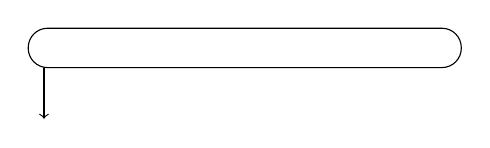
\begin{tikzpicture}\draw[rounded corners=7pt](0,0) rectangle(5.5,.5);\draw[->](.2,0)--(.2,-.65);\end{tikzpicture}}
\mspage{8}
